\documentclass{article}
\usepackage{amsfonts, amsmath, amssymb, amsthm, graphicx} % Math 
\graphicspath{ {./../images} }
\usepackage{enumitem}
\setlength{\parindent}{0pt} \oddsidemargin -0.2in \evensidemargin
0.0in \topmargin -1in \textheight 9.9in \textwidth 6.9in

\newtheorem{thm}{Theorem}
\newtheorem{prop}[thm]{Proposition}
\newtheorem{cor}[thm]{Corollary}
\newtheorem{claim}[thm]{Claim}

\newenvironment{problem}[2][Question]{\begin{trivlist}
\item[\hskip \labelsep {\bfseries #1}\hskip \labelsep {\bfseries #2.}]}{\end{trivlist}}

% main content
\begin{document} 

\textbf{Math 158 HW3}

% 3.8.9
\begin{problem}{3.8.9}
    Let $A_k$ be the set of subsets of $\{1,2, \dots , n\}$ of size $k$. Prove that for $k < n/2$, there is an injective function $f: A_k \rightarrow A_{k+1}$ such that $a \subseteq f(a)$ for all $a \in A_k$. For instance, if $k = 1$ and $n = 3$ then the function
    \[
        f(\{1\}) = \{1, 2\} \quad f(\{2\}) = \{2, 3\} \quad f(\{3\}) = \{1, 3\}
    \]
    is an example of such a function $f: A_1 \rightarrow A_2$.
\end{problem}

\begin{proof}
    Let $G$ be a bipartite graph with parts $A_k$ and $A_{k+1}$, for some $k < n / 2$, and each $a_k \in A_k$ forms an edge with $a_{k+1} \in A_{k+1}$ if $a_k \subset a_{k+1}$. We want to show that there is a matching saturating $A_k$. Since $k < n / 2$, $|A_k| = {n \choose k} \leq {n \choose k + 1} = |A_{k+1}|$. For each $a_k \in A_k$, there are $n - k$ number of $a_{k+1} \in A_{k+1}$ such that $a_k \subset a_{k+1}$, so each $a_k$ has $n - k$ neighbors. For each $a_{k+1} \in A_{k+1}$, there are $k + 1$ number of $a_k \in A_k$ such that $a_k \subset a_{k+1}$, so each $a_{k+1}$ has $k + 1$ neighbors. Since both sides are incident to the same number of edges, we know $(n - k)|A_k| = (k + 1)|A_{k+1}|$, and so $n - k \geq k + 1$ because $|A_k| \leq |A_{k+1}|$. Let $S \subseteq A_k$. We know there are $(n - k)|S|$ edges that are incident with $S$, and there are $(k + 1)|N(S)|$ edges that are incident with $N(S)$. Since the edges that are incident with $N(S)$ contain the ones that are incident with $S$, we have $(k + 1)|N(S)| \geq (n - k)|S| \geq (k + 1)|S|$, and so $|N(S)| \geq |S|$. Therefore, by Hall's Theorem, there is a matching saturating $A_k$ in $G$, which shows that there is an injection from $A_k$ to $A_{k+1}$.
\end{proof}

\newpage

% 3.8.17
\begin{problem}{3.8.17}
    An independent set in a graph G is a set $X \subseteq V (G)$ such that $e(X) = 0$, and the independence number $\alpha(G)$ is the largest size of an independent set in $G$. A vertex cover of $G$ is a set of vertices $X \subset V(G)$ such that $e \cap X \neq \emptyset$ for every edge $e \in E(G)$. The minimum size of a vertex cover of $G$, the vertex cover number, is denoted $\beta(G)$.
\end{problem}

\begin{enumerate}[label=(\alph*)]
    \item Prove that for any graph $G$, $\alpha(G) + \beta(G) = |V(G)|$.

    \begin{proof}
        Let $C$ be the smallest vertex cover of $G$, and let $I$ be the largest independent set in $G$. First, suppose that $|C \cup I| < |V(G)|$. Let $L = V(G) \backslash (C \cup I) \neq \emptyset$. Since there does not exist $e \in E(G)$ such that $e \subseteq V(G) \backslash C$, we know $e(L) = 0$. If $e(L \cup I) = 0$, then $L \cup I$ is a larger independent set, contradiction. So we can assume that for all $l \in L$, there exists $i \in I$ such that $\{l, i\} \in E(G)$. Then $I' = (I \backslash \{v\}) \cup \{u\}$ is also a largest independent set. This means that 
        we can find a largest independent set $I''$ such that $I'' \cup C = V(G)$. Therefore, we can assume $|C \cup I| = |V(G)|$. Suppose for the sake of contradiction that $C \cap I \neq \emptyset$. Let $v \in C \cap I$. Since $e(I) = 0$, we know $N(v) \subseteq V(G) \backslash I \subseteq C$. Since all neighbors of $v$ are in $C$, we can remove $v$ to get a smaller vertex cover $C \backslash \{v\}$, contradiction. Therefore, $C \cap I = \emptyset$, and thus $|V(G)| = |I \cup C| = |I| + |C| = \alpha(G) + \beta(G)$.
    \end{proof}

    \item  Prove that $\mu(G) \leq \beta(G) \leq 2\mu(G)$.
    
    \begin{proof}
        Let $M$ be the maximum matching of $G$, and $C$ be the smallest vertex cover. Since no two exposed vertices form an edge, the neighbors of exposed vertices are all saturated vertices, so the set of all saturated vertices is a vertex cover. Thus, $\beta(G) \leq 2\mu(G)$. If there exist $e \in M$ such that $e \cap C = \emptyset$, then $e$ is an uncovered edge, contradiction. Thus, for each edge $e \in M$, $e \cap C \neq \emptyset$, so $\mu(G) = |M| \leq \beta(G)$. Therefore, $\mu(G) \leq \beta(G) \leq 2\mu(G)$.
    \end{proof}
\end{enumerate}

\newpage

% 4.7.5
\begin{problem}{4.7.5}
    Determine which of the graphs in the figure below is planar. Justify your answers.
    
    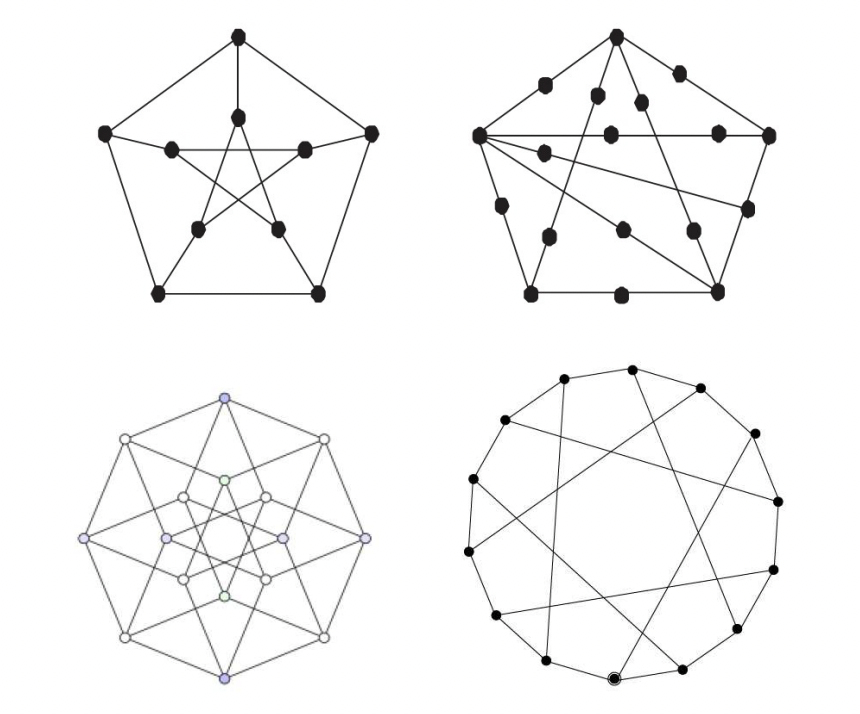
\includegraphics[width=.7\textwidth]{Q475}
\end{problem}

\begin{proof}[Solution]
    Since all four graphs have cycles, we can check by using the equation
    \[
        |E(G)| \leq \frac{g}{g - 2}(|V(G)| - 2),
    \]
    where $g$ is the length of the shortest cycle in the graph. 
    
    The graph on the top left has $15$ edges and $10$ vertices, and the shortest cycle has a length of $5$.
    \[
        15 > \frac{40}{3} = \frac{5}{5 - 2}(10 - 2),
    \]
    and thus it is not planar. 
    
    We can draw the graph on the top right in the following form:
    
    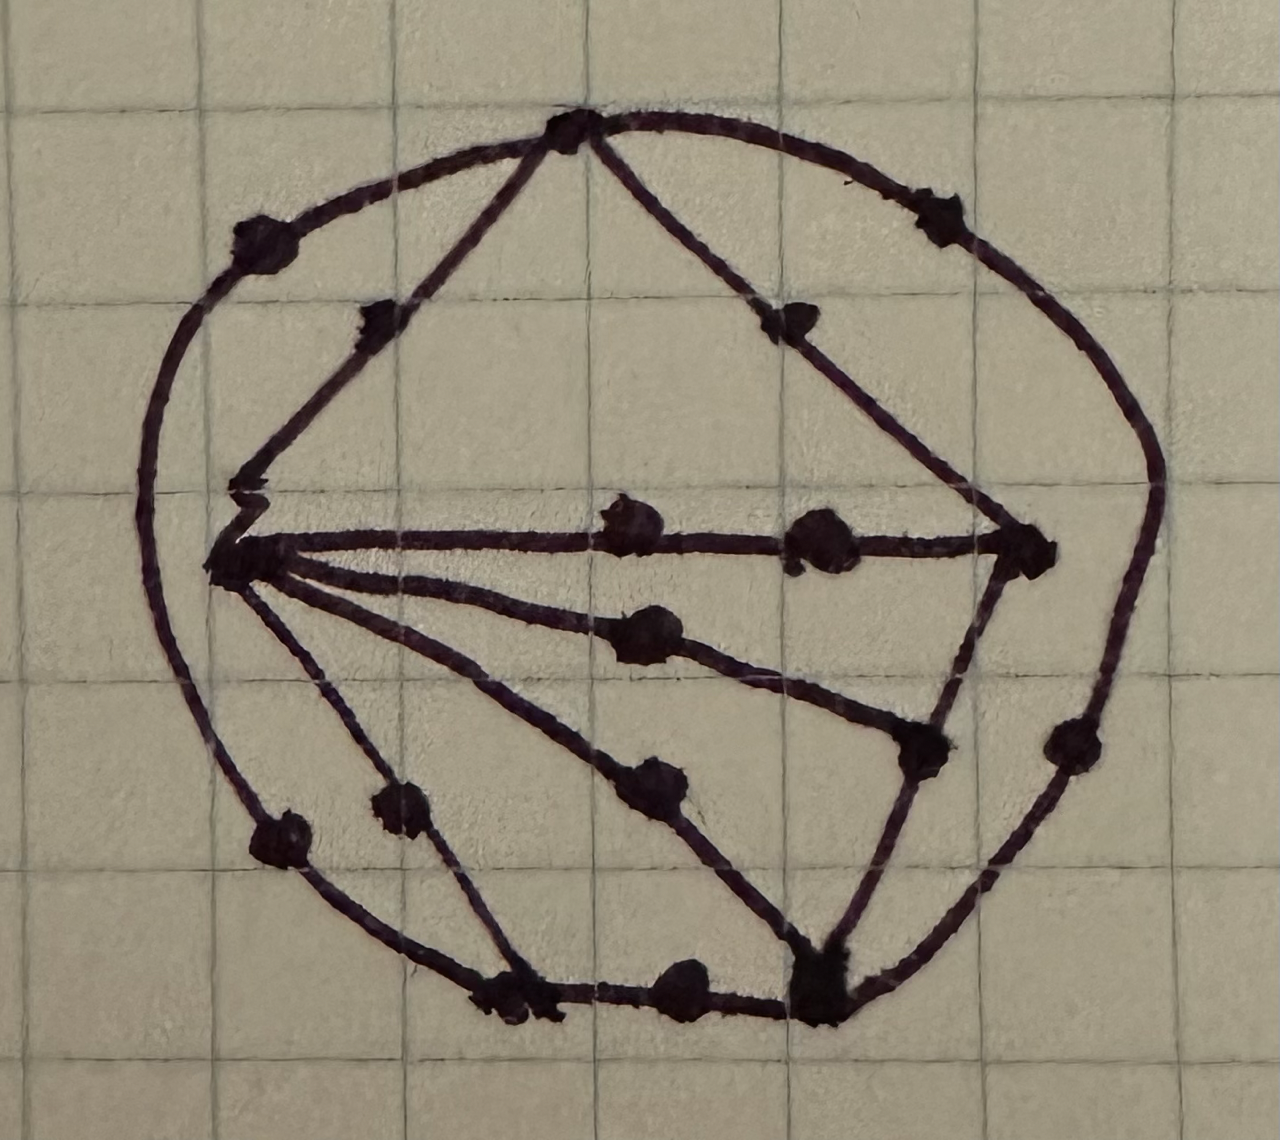
\includegraphics[width=.25\textwidth]{Q475-2} \\
    Therefore, the graph is planar.

    The graph on the bottom left has $32$ edges and $16$ vertices, and the shortest cycle has a length of $4$.
    \[
        32 > 28 = \frac{4}{4 - 2}(16 - 2),
    \]
    and thus it is not planar. 

    The graph on the bottom right has $20$ edges and $14$ vertices, and the shortest cycle has a length of $6$.
    \[
        20 > 18 = \frac{6}{6 - 2}(14 - 2),
    \]
    and thus it is not planar. 
\end{proof}

\newpage

% 4.7.7
\begin{problem}{4.7.7}
    A maximal plane graph is a plane graph $G = (V, E)$ with $n \geq 3$ vertices such that if we join any two non-adjacent vertices in $G$, we obtain a non-plane graph
\end{problem}

\begin{enumerate}[label=(\alph*)]
    \item Draw a maximal plane graph on six vertices.

    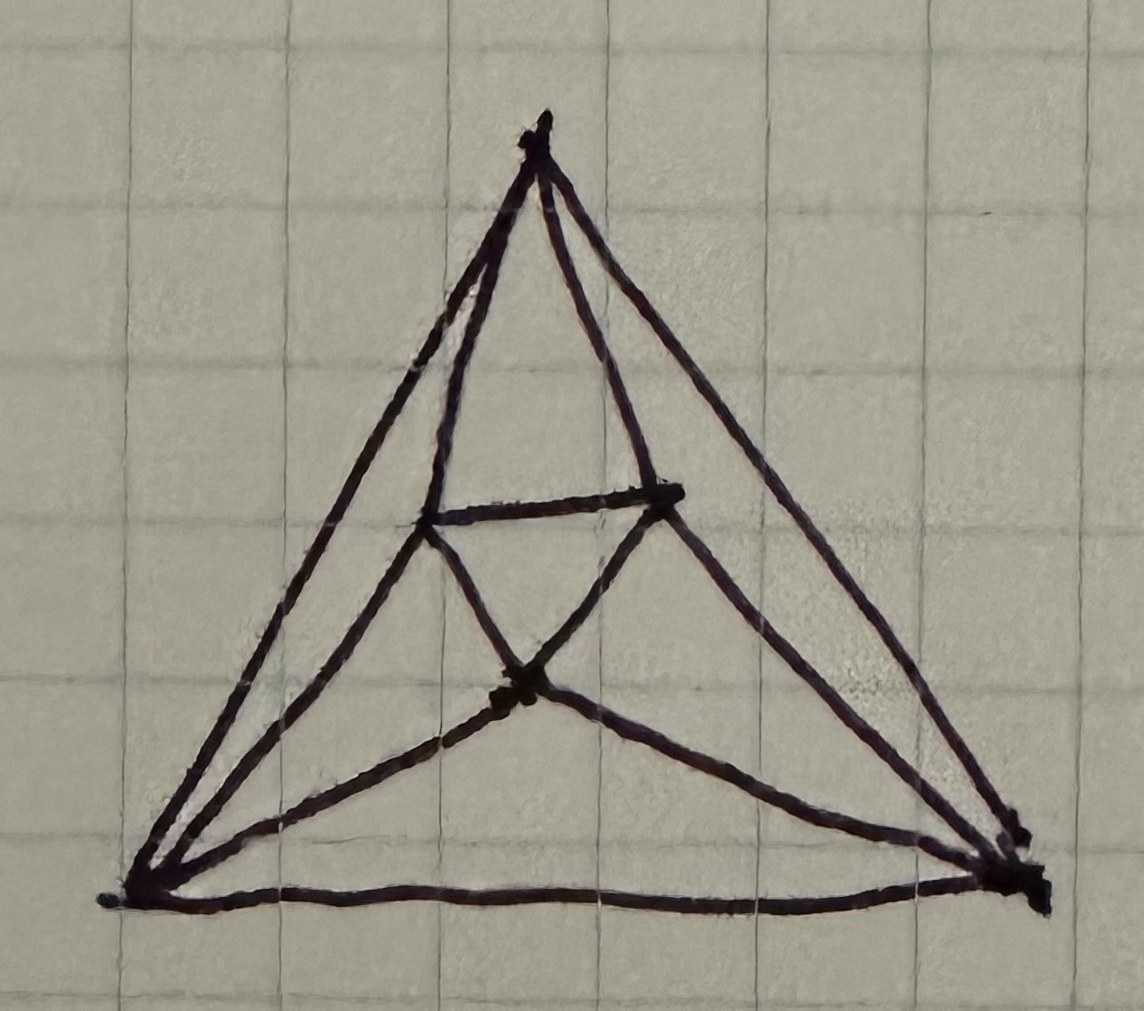
\includegraphics[width=.25\textwidth]{Q477a}

    \item Show that a maximal plane graph on $n$ points has $3n - 6$ edges and $2n - 4$ faces.

    \begin{proof}
        A maximal plane graph $G$ only contains faces with degree $3$. $G$ is connected because if it's not, we can add an edge to connect two components and still get a plane graph, which contradicts $G$'s maximality. By Handshake Theorem for faces, we know $3|F(G)| = \sum\limits_{f \in F(G)} deg(f) = 2|E(G)|$. By Euler's Formula, we have $|V(G)| - |E(G)| + |F(G)| = n - |E(G)| + \frac{2}{3}|E(G)| = 2$, and thus $|E(G)| = 3n - 6$, $|F(G)| = \frac{2}{3}|E(G)| = 2n - 4$.
    \end{proof}
    
    \item A triangulation of an $n$-gon is a plane graph whose vertex set is the vertex set of a convex $n$-gon in the plane, whose infinite face boundary is a convex $n$-gon, and all of whose other faces are triangles. How many edges does a triangulation of an $n$-gon have?
    
    \begin{proof}[Solution]
        To triangulate a $n$-gon, we can pick a vertex $v$ from the $n$-gon and connect it with all other vertices in the graph. Since $v$ is already connected to two vertices, we only need to add $n - 1 - 2 = n - 3$ edges. Therefore, including the original $n$ edges, a triangulation of an $n$-gon has $2n - 3$ edges.
    \end{proof}
\end{enumerate}

\newpage

% 4.7.14
\begin{problem}{4.7.14}
    Let $\omega(G)$ – the clique number of $G$ – be the maximum number of vertices in a complete subgraph of a graph $G$.
\end{problem}

\begin{enumerate}[label=(\alph*)]
    \item Prove that for every graph $G$, $\chi(G) \geq \omega(G)$.

    \begin{proof}
        We know that $\chi(K_n) = n$. Since $K_{\omega(G)} \subseteq G$, we need at least $n$ colors to color $G$, so $\chi(G) \geq \omega(G)$.
    \end{proof}

    \item Prove that for every graph $G$, $\chi(G) \geq |V(G)|/\alpha(G)$.

    \begin{proof}
        Suppose that we color $G$ with $\chi(G)$ colors. Since no vertices with the same color form an edge, each set of vertices with the same color is an independent set and has a size less than $\alpha(G)$, and there are $\chi(G)$ of them. Therefore, $\alpha(G)\chi(G) \geq |V(G)|$, and, rearranged, we get $\chi(G) \geq |V(G)| / \alpha(G)$
    \end{proof}
    
    \item For each $k \geq 2$, find a graph $G$ such that $\chi(G) = k + 1$ and $\omega(G) = k$.
    
    \begin{proof}[Solution]
        For $k = 2$, a length $5$ cycle has $\omega(G) = k$ and $\chi(G) = k + 1$. For $k > 2$, we can start from a $k$-complete graph $F$ with a vertex set $\{s_1, s_2, \dots, s_k\}$, each colored differently with the set of colors $C = \{c_1, c_2, \dots, c_k\}$. Let $H = (V(F) \cup V, E(F) \cup E)$, where $V = \{b_1, b_2, \dots, b_k\}$ and $E = \{\{b_i, s_j\} : b_i \in V, \, s_j \in V(F), \, i \neq j\}$. Since each $b_i \in V$ is connected to $k - 1$ vertices of different colors in $H$, we color $b_i$ with the only available color in $C$, and now $b_i$ has the same color as $s_i$. We then add a vertex $v$ to $H$ and let $v$ form an edge with each $b_i \in V$, and we call this graph $G$. Since all $b_i \in V$ are colored differently, $v$ has $k$ neighbors with $k$ different colors, so $v$ must be colored by a new color. Since $N(v) = V$, no two neighbors of $v$ are connected to each other. We also know that $v$ does not have an edge with any of the vertices in $F$. Thus, we can assume if there is a $K_{k+1}$ in $G$, $V(F) \cup \{b_i\} = V(K_{k+1})$, for some $b_i \in V$. However, $b_i$ does not form an edge with all vertices in $F$. Thus, $G$ does not contain $K_{k+1}$. Therefore, we get a graph $G$ where $\chi(G) = k + 1$ and $\omega(G) = k$. 
    \end{proof}

    Below is an illustration of what $G$ looks like when $k = 5$.

    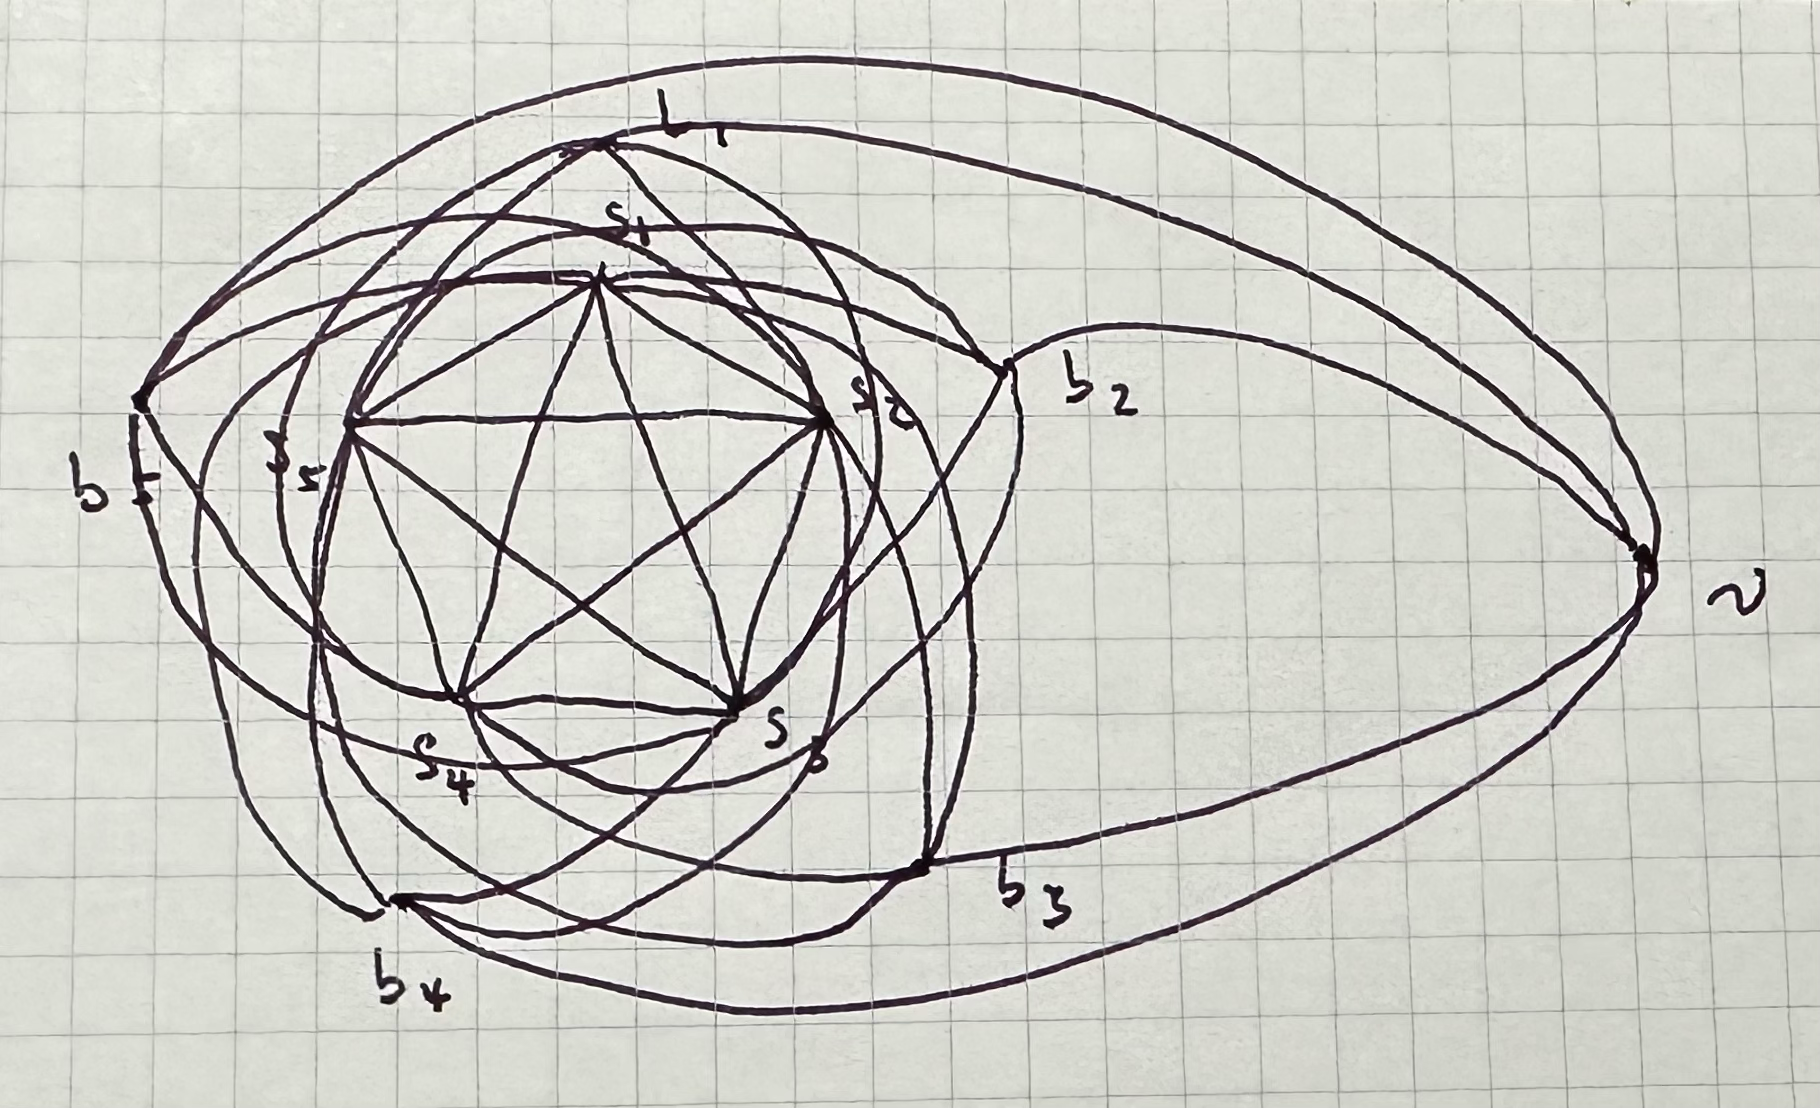
\includegraphics[width=.7\textwidth]{Q4714}
\end{enumerate}

\end{document}